\section{Theory of flat curved systems}\label{sec:theory_1D}

The theoretical description of the time evolution of magnetization distribution in curved systems is based on the solution of the phenomenological Landau--Lifshitz--Gilbert (LLG) equation of motion~\cite{Landau35,Gilbert04}
\begin{equation}\label{eq:llg}
\frac{\mathrm{d}\vec{m}}{\mathrm{d}t}=\underbrace{-\gamma_0\, \vec{m}\times\vec{H}_\textrm{eff}}_{\text{Precession term}} + \underbrace{\alpha_\textsc{g}\, \vec{m}\times\frac{\mathrm{d}\vec{m}}{\mathrm{d}t}}_{\text{Damping term}},
\end{equation}
which defines the damped precession motion of the unit magnetization vector, $\vec{m}=\vec{M}/M_s$, with $M_s$ being a saturation magnetization, around an effective magnetic field, $\vec{H}_\textrm{eff}=-\delta E/\delta\vec{M}$, that is derived as functional derivative of the total micromagnetic energy, $E$. In Eq.~\eqref{eq:llg}, $\gamma_0$ is the gyromagnetic ratio and $\alpha_\textsc{g}$ is the Gilbert damping parameter~\cite{Gilbert04}.



\subsection{Model of curved 1D magnetic system}\label{sec:model_1D}

Without losing generality, let us consider the prototypical case of a curvilinear anisotropic one-dimensional Heisenberg nanomagnet, which is determine in the Cartesian frame of reference by a three-dimensional curve, $\vec{\gamma}=\vec{\gamma}(s)$, with natural parameter, $s$. The total energy of such magnet includes energies of exchange interaction, $E_\textrm{ex}$, and uniaxial magnetic anisotropy, $E_\textrm{an}$,
\begin{equation}\label{eq:total_energy}
E=E_\textrm{ex} + E_\textrm{an} =\int\mathrm{d}\vec{r}\, \left[A \, (\nabla m_i)(\nabla m_i)-K \, (\vec{m}\cdot \vec{e}_\mathrm{A})^2 \right].
\end{equation}
Here and below we will use the Einstein summation convention with $i = x,\,y,\,z$. The first term in Eq.~\eqref{eq:total_energy} describes the isotropic exchange interaction with $A$ being the exchange stiffness constant~\cite{Brown63}, while the second term corresponds to the magnetic anisotropy with $K$ and $\vec{e}_\mathrm{A}$ being the constant and the direction of the uniaxial anisotropy, respectively. The competition between exchange and anisotropy results in the magnetic length $\ell=\sqrt{A/K}$, which determines a length scale of the system.

In the case of an arbitrary curved magnetic wire and tangential direction of the anisotropic easy-axis, $K>0$ and $\vec{e}_\mathrm{A} = \vec{e}_\mathrm{T}$, the consideration of magnetic anisotropy becomes non-trivial due to the coordinate-dependence of its term in Eq.~\eqref{eq:total_energy}. Therefore, it is instructive to introduce a local curvilinear frame of reference, the transition to which allows to restore the translation-invariant form of $E_\textrm{an}$ and get rid of the coordinate dependence in the anisotropy term. In the case of one-dimensional systems, it is convenient to use the Frenet-Serret reference frame  
\begin{equation} \label{eq:Frenet-Serret}
		\vec{e}_\mathrm{T} = \vec{\gamma}', \qquad  \vec{e}_\mathrm{N} = \dfrac{\vec{\gamma}''}{\kappa} , \qquad  \vec{e}_\mathrm{B} = \vec{e}_\mathrm{T} \times \vec{e}_\mathrm{N},
\end{equation}
where $\vec{e}_\textrm{T}$, $\vec{e}_\textrm{N}$, and $\vec{e}_\textrm{B}$ are the tangential, normal, and binormal unit vectors, respectively~\cite{Kreyszig91}, see Fig.~\ref{fig:TNB}. Here prime denotes the derivative with respect to the natural parameter, $s$, and $\kappa = |\vec{\gamma}''|$  is a local arc curvature. The relation between $\partial_{s} \vec{e}_{\alpha}$ and $\vec{e}_{\alpha}$ is determined by the Frenet-Serret formulas~\cite{Kreyszig91}:
\begin{equation} \label{eq:Darboux_vector}
	\vec{e}_{\alpha}' = \mathcal{F}_{\alpha \beta} \, \vec{e}_{\beta}, \qquad \begin{Vmatrix} \mathcal{F}_{\alpha \beta} \end{Vmatrix} = \left(\begin{matrix*} \, 0 \quad	& \kappa \quad &  0 \, \, \, \\ \, -\kappa \quad & 0 \quad & \tau \, \, \, \\
	\, 0 \quad & -\tau \quad &	0 \, \, \,
	\end{matrix*}\right),	
\end{equation}
whereas Greek indices $\alpha,\, \beta = \textrm{T},\, \textrm{N},\, \textrm{B}$ enumerate the curvilinear coordinates and the curvilinear components of vector fields, $\kappa(s)$ and $\tau(s)$ are local curvature and torsion of the wire, respectively. Using the introduced Frenet--Serret frame of reference it is now possible to parameterize physical wires or stripes with a finite cross section as
\begin{equation} \label{eq:Stripe_param}
\vec{r}\left(s,\zeta_1,\zeta_1\right)=\vec{\gamma}(s) + \zeta_1 \, \vec{e}_\textsc{n}+\zeta_2 \, \vec{e}_\textsc{b},
\end{equation}
where $\zeta_i$ are coordinates within the cross section, see Fig.~\ref{fig:TNB}. In the case when $\sqrt{\zeta_1^2+\zeta_2^2}\leq \ell$, the magnetic object can be treated as a one-dimensional system and formalized as $\vec{m}=\vec{m}(s)$.

%==================================================================\
\begin{figure}[t]
	\centering
	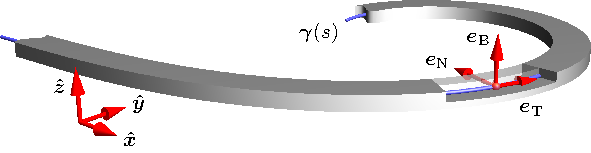
\includegraphics[width=0.7\textwidth]{TNB_basis_1}
	\caption{\label{fig:TNB}%
		\textbf{Schematics of Frenet-Serret basis for flat curvilinear geometries.} Geometrical construction of a flat curved system from a one-dimensional wire $\vec{\gamma}(s)$ by using geometrical expansion along normal $\vec{e}_\textrm{N}$ and binormal $\vec{e}_\textrm{B}$ directions. Adapted with permission from~\cite{Yershov18a}.
	}
\end{figure}
%==================================================================/

Applying the Frenet-Serret apparatus~\eqref{eq:Darboux_vector} to any kind of curved one-dimensional magnetic nanowire leads to the restoring of the translational-invariant form of magnetic anisotropy and restructuring all magnetic energy terms containing spatial derivatives. In the case of the one-dimensional Heisenberg nanomagnet with the total energy~\eqref{eq:total_energy}, the exchange interaction is becoming a characteristic example of such geometrical transformation: in the curvilinear reference frame~\eqref{eq:FrenetSerret_basis} with the magnetization parametrization $\vec{m} = m_\textrm{T}\,\vec{e}_\textrm{T} + m_\textrm{N}\,\vec{e}_\textrm{N} + m_\textrm{B}\,\vec{e}_\textrm{B}$, the exchange energy reads as~\cite{Sheka15}:
\begin{equation} \label{eq:Exchange_energy_TNB_1}
E_{\textrm{ex}} = S \, \int \textrm{d} s  \, \, A \left[ \left| \vec{m}' \right|^2 + \mathcal{F}_{\alpha \beta} \, ( m_{\alpha} \, m'_{\beta} - m'_{\alpha} \, m_{\beta} ) + \mathcal{K}_{\alpha \beta} \, m_{\alpha} \, m_{\beta} \right],
\end{equation}
where $S$ is the cross section area of the nanomagnet. The first term is the isotropic part of the exchange which formally  has the same form as for a straight wire. The second term in \eqref{eq:Exchange_energy_TNB_1} is the chiral term, which has the set of the Lifshitz invariants and describe the geometrical symmetry breaking. This set of the Lifshitz invariants in the curvilinear frame of reference can be referred to a curvature-induced Dzyaloshinskii-Moriya interaction (DMI), which is linear with respect to local curvature $\kappa(s)$ and torsion $\tau(s)$. The third term in \eqref{eq:Exchange_energy_TNB_1} describes the curvature-induced anisotropy. The corresponding coefficients are determined by the components of the tensor $\mathcal{K}_{\alpha \beta}= \mathcal{F}_{\alpha \nu} \, \mathcal{F}_{\beta \nu}$. They are bilinear with respect to local curvature, $\kappa$, and torsion, $\tau$:
\begin{equation} \label{eq:K_tensor_exchange}
\begin{Vmatrix} \mathcal{K}_{\alpha \beta} \end{Vmatrix} = \left(\begin{matrix*}  \, \kappa^2 \quad	& 0 \quad & - \kappa \, \tau \, \,  \\
\, 0 \quad & \kappa^2 + \tau^2 \quad & 0 \, \,  \\
\, - \kappa \, \tau \quad & 0 \quad &	\tau^2 \, \, 
\end{matrix*}\right).
\end{equation}
It is also convenient to represent the exchange energy \eqref{eq:Exchange_energy_TNB_1} in the following form:
\begin{equation} \label{eq:Exchange_energy_TNB_2}
E_{\textrm{ex}} =  S \, \int \textrm{d} s \, \, A \left| \vec{m}' \right|^2 - S \int \textrm{d} s \, \, \vec{D}^{\scriptsize \textsc{e}} \cdot [\vec{m} \times \vec{m}'] - S \int \textrm{d} s \, \, A \left[ \tau \, m_{\scriptsize \textsc{t}}  + \kappa \, m_{\scriptsize \textsc{b}} \right]^2, 
\end{equation}
where the property $|\vec{m}|=1$ and Frenet-Serret formulae are utilized. In the \eqref{eq:Exchange_energy_TNB_2}, vector $\vec{D}^{\scriptsize \textsc{e}} = - 2 \, A \, \tau \, \vec{e}_{\scriptsize \textsc{t}} - 2 \, A \, \kappa \, \vec{e}_{\scriptsize \textsc{b}}$ denotes the reduced vector of the \textit{extrinsic} curvature-driven DMI~\cite{Gaididei14,Sheka15,Sheka15c}.	In contrast to the \textit{intrinsic} DMI, which comes from the spin-orbit coupling in bulk magnetic crystals with low symmetry~\cite{Dzyaloshinsky58,Moriya60a} or at interfaces between a ferromagnet and a nonmagnetic material with strong spin-orbit coupling~\cite{Fert90,Crepieux98,Bode07,Yang15}, the strength of \textit{extrinsic} DMI is determined by local curvature and torsion~\cite{Pylypovskyi16,Volkov19c}. The vector of the \textit{extrinsic} DMI is always lying in the rectifying plane to a curved geometry~\cite{Volkov18}.

%==================================================================\
\begin{figure}[t]
	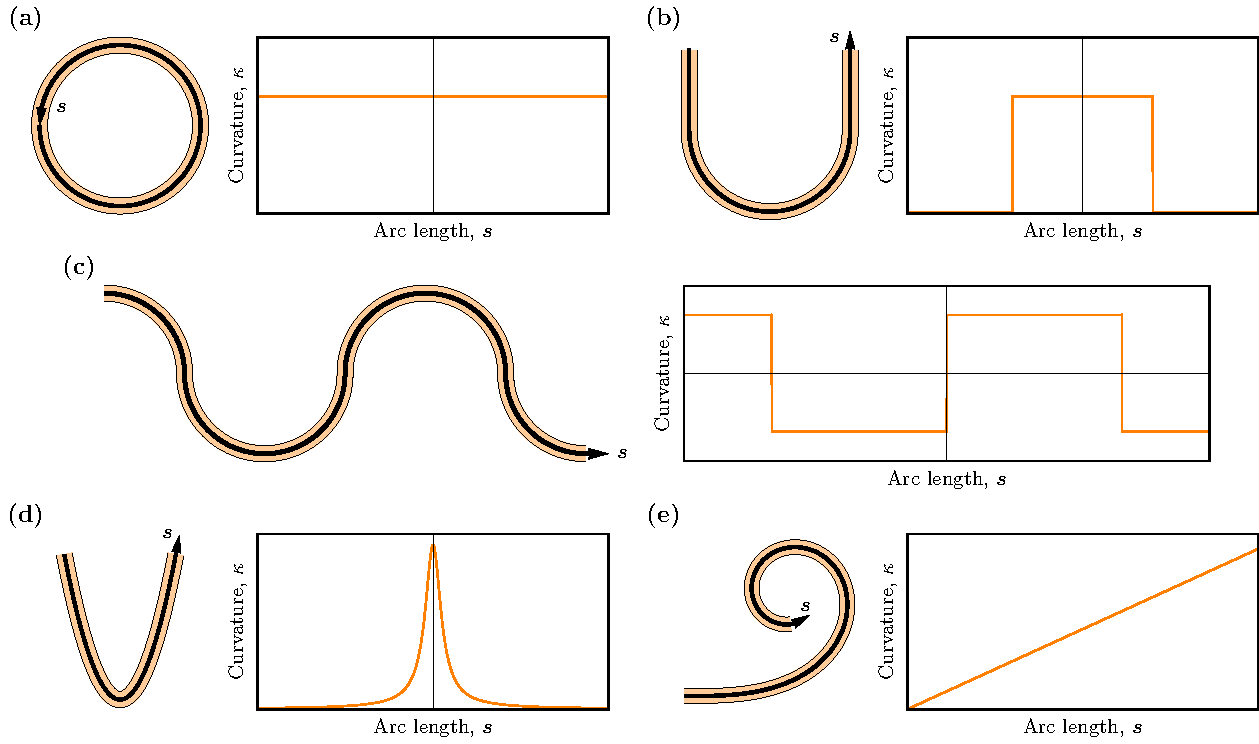
\includegraphics[width=\textwidth]{Geometries_n_curvatures_1}
	\caption{\label{fig:Geometries_n_curvatures}%
		\textbf{Schematics of flat curvilinear geometries and their curvature distributions.} \textbf{(a),} Circular ring with constant $\kappa = 1/R = \textrm{const}$, where $R$ is a ring radius. \textbf{(b)}, Nanostripe with individual circular segment, which correspond to the box-function spatial profile of curvature: $\kappa = \kappa_0$ when $-s_0\leq s \leq s_0$ and $\kappa = 0$ elsewhere. \textbf{(c)}, Meander-like nanowire constructed from repeated semicircles of same radius $R$. The spatial distribution of the curvature of such a wire is the square-wave function $\varkappa(\xi) = (-1)^{\lfloor\xi/\xi_0\rfloor}\varkappa_0$ with period $2\xi_0$, $\xi_0=\pi/\varkappa_0$, and $\lfloor x \rfloor$ defines the integer part of $x$. \textbf{(d)}, Parabolic nanostripe with localized curvature gradient. \textbf{(e)}, Euler spiral and constant non-zero curvature gradient along the stripe. }
\end{figure}
%==================================================================/

In the present Chapter, we will limit ourselves to the description of various flat curvilinear magnetic geometries and corresponding curvature-induced effects in them ($\tau=0$ and $\vec{e}_\textrm{B} = \vec{\hat{\vec{z}}}$). Magnetic effects associated with presence of curvature and torsion in three-dimensional curvilinear magnetic systems will be discussed in the following \textcolor{red}{Chapters}. Therefore, it is instructive to address the impact of curvature on magnetic subsystem for different flat curvilinear geometries with distinct curvature distributions:
\begin{itemize}
	\item \textbf{Nanorings} as geometries with constant curvature ($\kappa = \kappa_0 = \textrm{const}$);
	\item \textbf{Nanowire with circular segment} and box-function curvature profile ($\kappa = \kappa_0$ when $-s_0\leq s \leq s_0$ and $\kappa = 0$ elsewhere);
	\item \textbf{Meander-like shape nanowire} with the square-wave curvature distribution;
	\item \textbf{Parabolic nanowires} with localized curvature gradient;
	\item \textbf{Spirals} with non-zero curvature gradient along the stripe.
\end{itemize}


